% 
% Annual Cognitive Science Conference
% Sample LaTeX Paper -- Proceedings Format
% 

% Original : Ashwin Ram (ashwin@cc.gatech.edu)       04/01/1994
% Modified : Johanna Moore (jmoore@cs.pitt.edu)      03/17/1995
% Modified : David Noelle (noelle@ucsd.edu)          03/15/1996
% Modified : Pat Langley (langley@cs.stanford.edu)   01/26/1997
% Latex2e corrections by Ramin Charles Nakisa        01/28/1997 
% Modified : Tina Eliassi-Rad (eliassi@cs.wisc.edu)  01/31/1998
% Modified : Trisha Yannuzzi (trisha@ircs.upenn.edu) 12/28/1999 (in process)
% Modified : Mary Ellen Foster (M.E.Foster@ed.ac.uk) 12/11/2000
% Modified : Ken Forbus                              01/23/2004
% Modified : Eli M. Silk (esilk@pitt.edu)            05/24/2005
% Modified : Niels Taatgen (taatgen@cmu.edu)         10/24/2006
% Modified : David Noelle (dnoelle@ucmerced.edu)     11/19/2014
% Modified : Roger Levy (rplevy@mit.edu)     12/31/2018



%% Change "letterpaper" in the following line to "a4paper" if you must.

\documentclass[10pt,letterpaper]{article}

\usepackage{cogsci}
\usepackage{color}
\usepackage{graphicx}
\graphicspath{{figs/}}
%\cogscifinalcopy % Uncomment this line for the final submission 


\usepackage{pslatex}
\usepackage{apacite}
\usepackage{float} % Roger Levy added this and changed figure/table
                   % placement to [H] for conformity to Word template,
                   % though floating tables and figures to top is
                   % still generally recommended!

%\usepackage[none]{hyphenat} % Sometimes it can be useful to turn off
%hyphenation for purposes such as spell checking of the resulting
%PDF.  Uncomment this block to turn off hyphenation.


%\setlength\titlebox{4.5cm}
% You can expand the titlebox if you need extra space
% to show all the authors. Please do not make the titlebox
% smaller than 4.5cm (the original size).
%%If you do, we reserve the right to require you to change it back in
%%the camera-ready version, which could interfere with the timely
%%appearance of your paper in the Proceedings.

\providecommand{\tightlist}{%
  \setlength{\itemsep}{0pt}\setlength{\parskip}{0pt}}
  
\definecolor{Red}{RGB}{255,0,0}
\definecolor{Green}{RGB}{10,200,100}
\definecolor{Blue}{RGB}{10,100,200}

\newcommand{\mh}[1]{{\textcolor{Blue}{[mh: #1]}}}
\newcommand{\rl}[1]{{\textcolor{Green}{[roger: #1]}}}

\newcommand{\denote}[1]{\mbox{ $[\![ #1 ]\!]$}}
\newcommand{\red}[1]{{\textcolor{Red}{#1}}}

\title{Syntactic expectations modulate pragmatic interpretations of generic sentences}
 
\author{{\large \bf Michael Henry Tessler (tessler@mit.edu)} \\
  Department of Brain and Cognitive Sciences, MIT \\
  Cambridge, MA 02139 USA
  \AND {\large \bf Roger Levy (rplevy@mit.edu)} \\
  Department of Brain and Cognitive Sciences, MIT \\
  Cambridge, MA 02139 USA}


\begin{document}

\maketitle


\begin{abstract}

A hallmark of human thinking is our ability to update ours beliefs in the face of conflicting evidence. 

\textbf{Keywords:} 
semantics; pragmatics; incremental processing; generics
\end{abstract}


\section{Introduction}

Much of what we come to learn about the world comes not from direct experience but from knowledge conveyed to us from others, often in the form of linguistic utterances. 
``Elephants eat 300 pounds of a food in a day'' succinctly conveys information that extends beyond any particular moment in time or space (e.g., it could apply to any elephant, any day of the week). 
Utterances that communicate generalizations are called \emph{generic} utterances \cite{Carlson1977, genericBook}, and they are the foremost case study of rich, abstract knowledge conveyed in simple utterances \cite{Gelman2009}.
%Understanding how generic language updates beliefs holds the key to understanding how young children build rich, intuitive theories \cite{Gelman2009}. 

Understanding generic language pose a number of philosophical challenges that have made it very difficult to develop a unified, formal theory of their meaning \cite<for useful reviews, see:~>{genericBook, Leslie2008, Nickel2016}. 
A simple theory that generics mean something analogous to \emph{most} \cite<e.g., ``Most elephants eat 300 pounds of food in day''; >{Cohen1999} has trouble accounting for generics about conjunctive, mutually-exclusive properties. 
``Elephants live in Africa and Asia'' is true despite no elephant living in both; the sentence should be understood as ``Elephants live in Africa, and elephants live in Asia'', but this is impossible if each individual generic sentence means something analogous to \emph{most} \cite{Nickel2008}.

%The sentence ``Robins lay eggs'' is true despite the property only applying to female robins, yet the same logic does not make ``Robins are female'' a true or felicitous utterance. 


%Crucially, this theory posits that the meaning of a generic is uncertain one which can be updated as more information is available.

The puzzle of understanding conjunctive generic sentences deepen when one considers that actual linguistic input needs to be processed incrementally: Listeners may start forming expectations about the intended meaning before the speaker finishes their sentence. 
Listeners comprehend sentences incrementally, making use of moment to moment linguistic input in order to make predictions about future input \cite<e.g.,>{Altmann1999}.
The sentence  ``Elephants live in Africa and Asia'', thus, at some point is heard as just ``Elephants live in Africa'', which could imply a different meaning than the sentence as a whole.


Here, we combine a recent model of generic language understanding  \cite{Tessler2019:genLang} with an incremental parsing mechanism to begin to form beliefs about a speaker's intended meaning before the speaker has finished speaking.
The basic, non-incremental model understands ``Elephants live in Africa and Asia” as meaning that some elephants live in Africa and that different ones live in Asia, in the case where listeners have prior knowledge suggesting against the existence of elephants that live on both continents (\emph{international elephants}).
Furthermore, the enriched incremental model makes the prediction that part-way through generic sentences about conjunctive predicates (e.g., ``Elephants live in Africa''), a listener will form strong beliefs (i.e., \emph{all elephants live in Africa}) which later get non-monotonically updated once more information comes in (\emph{some live in Africa and some live in Asia}).
We test this prediction in a set of language understanding tasks where participants are asked to report their beliefs about the prevalence of a property in a category at different points in a sentence, analogous to gating paradigms in psycholinguistics \cite{Grosjean1980}.


%Recently, \cite{Tessler2019:genLang} proposed a theory of generic language wherein the meaning of a generic is \emph{underspecified} (or, vague) and Bayesian reasoning is used to resolve more precise meanings in context.


%Intriguingly, this model also predicts that (i.e., upon hearing only that ``Elephants live in Africa'') leads our model to believe that most, possibly all, elephants live in Africa, but when the sentence is completed (``. . . and Asia''), the model nonmonotonically updates its beliefs to the weaker \emph{some elephants live in Africa and others in Asia}. 


%Interpreting generics in a consistent way is a non-starter. 


%Theories that appeal to standard, formal semantic, quantificational truth conditions (e.g., generic means \emph{most} or \emph{all} relevant or normal members of the category have the property) employ mechanisms to implicitly restrict the \emph{relevant} set of robins to be females in the case of a property concerning reproduction such as \emph{laying eggs}\cite<e.g.,>{Cohen1999}. 
%(such as that of  where a generic ``Ks F'' means roughly that \emph{most of the relevant Ks F})

%Interpreting generics in a 
%Such restrictions, however, are too limiting when interpreting conjunctive predicates as in ``Elephants live in Africa and Asia''. 
% from knowledge about the kind of property under consideration (i.e., \emph{laying eggs} has to do with reproduction, so we are only talking about females), but this mechanism is too restrictive when it comes to generics about conjunctive properties such as ``Elephants live in Africa and Asia'': 
%It cannot be the case that most (more than half of) elephants live in Africa and most (more than half of) elephants live in Asia, unless we imagine elephants migrating back-and-forth from continent to continent (i.e,. \emph{international elephants}), which is intuitively implausible \cite{Nickel2008}.
%More generally, a theory of generics need be sufficiently flexible to accommodate property-specific interpretations (e.g., ``Robins lay eggs'' means half of robins lay eggs; ``Dogs get cancer'' means some dogs get cancer; ``Birds fly'' means almost all birds fly) as well as be able to revise those interpretations with new, potentially conflicting evidence (e.g., consider ``Elephants live in Africa''~vs.~``Elephants live in Africa and Asia'').



%``Lions have manes and give live birth'' wherein the first and second conjuncts apply to distinct subsets (i.e., male lions have manes and female lions give live birth).



%Consider the following examples:
%
%\begin{enumerate}
%\tightlist
%\item Triangles have three sides and three angles.
%\item Ravens have two wings and two legs.
%\item Elephants live in Africa and Asia.
%\item Lions have manes and give live birth.
%\end{enumerate}
%
%It is conceivable that both (1) and (2) can be analyzed in terms of a (context-sensitive) generic operator acting on a logically complex predicates (i.e., \emph{all triangles both have three sides and three angles}, \emph{most ravens have two wings and two legs}). 
%Individual elephants do not migrate across continents and thus live in both Africa and Asia. 
%The individual lions that have manes are a distinct sub-category from those that give live birth (i.e., the properties pick out the males and the females, respectively). 
%The logically complex predicates in sentences (3) and (4), thus, are not true generically of their associated categories; rather, the sentences should be understood as a conjunction of generic sentences.

\section{Computational Model}

We extend the generic interpretation model of \citeA{Tessler2019:genLang} to incorporate an incremental processing mechanism that allows a listener to understand meaningful chunks of a full utterance.
The basic model interprets a generic utterance predicating a property of a category (``Elephants eat 300 pounds of food in a day'') as meaning that the \emph{prevalence} $x$ or probability of the property given the category---$P($eats 300 lb. of food in a day$\mid$ is an elephant$)$---is greater than an \emph{a priori} uncertain threshold $\theta$. 
The literal meaning of the generic---an uncertain threshold function---combines with a listener's prior knowledge about the prevalence of the feature $P(x)$ within a relevant set of alternative categories (e.g., other animals) to compute a posterior distribution over prevalence $x$. 
\begin{equation}
P(x \mid u) = \int_{\theta} P(x, \theta \mid u)  d\theta \propto P(x) \cdot P(\theta) \cdot \delta_{\denote{u}(x, \theta)} 
\label{eq:L0}
\end{equation}
\noindent where $\delta_{\denote{u}(x, \theta)}$ is the Kronecker delta function assigning a value of 1 for utterances that are literally true (in the case of a generic: where $x > \theta$) and 0 for utterances that are false.

Equation \ref{eq:L0} is a model of a Bayesian listener interpreting a complete utterance.
Listeners may begin to form expectations about the complete utterance even before the sentence is over. 
For example, in the case of interpreting a generic sentence about a conjunctive property (e.g., ``Elephants live in Africa and Asia''), a listener is given the opportunity to form a partial, plausible interpretation of the utterance by the time they read the first conjunct (``Africa''). 
In order to model incremental interpretations of the utterance, we extend this model to allow a listener to form expectations about plausible continuations from sentence fragments $f$.
To do this, we assume that a listener has probabilistic expectations about how a speaker will choose to complete the utterance given a fragment $P(u' \mid f)$.

\begin{equation}
P(x \mid f) = \sum_{u'}) P(x \mid u') P(u' \mid f) 
\label{eq:L0a}
\end{equation}

We consider the case of listeners encountering the coordinating connection ``and'' \red{in the predicate(?) position of a generic sentence}. 
For simplicity, we assume that speakers can continue a sentence such as ``Elephants live in Africa and'' with either an NP coordination with a mutually exclusive property (``Asia'') or VP coordination with a non-mutually exclusive property (``eat 300 pounds of food a day'').\footnote{
	Of course, NP-coordination with non-mutually exclusive properties is possible (e.g., ``eat figs and nuts''). 
	Our focus in this paper is on the fact that a speaker can continue the conjunction with a mutually exclusive or non-mutually exclusive property, which in the cases we consider, are perfectly correlation with NP~vs.~VP coordination.
}


%Extending an analysis of generics to handle complex-predicates poses unique challenges.
%A sentence of the form ``Ks F and G'' introduces an ambiguity:
%
%\begin{enumerate}
%\tightlist
%\item $\denote{gen}(K) [F \land G]$
%\item $\denote{gen}(K) [F] \land \denote{gen}(K) [G]$
%\end{enumerate}


\section{Experiments}

We design three experiments to test the mutual exclusivity (ME) and incremental predictions of the model. 
Experiment 1 tests the basic ME predictions that ``Elephants live in Africa and Asia'' means roughly that half live in Africa and half live in Asia; we control for this using generics with conjunctive, non-mutually exclusive (NME) properties (e.g., ``Elephants live in Africa and eat 300 lb. of food in a day''). 
Experiment 2 is a conceptual replication using an adaptation of a gating paradigm \cite{Grosjean1980} which also controls for asking about two properties previously mentioned using a conjunctive generic sentence. 
Experiment 3 also uses the gating paradigm to test the fine-grained incremental predictions of the model.
Sample size, participant exclusion criteria, and primary planned analyses for all experiments were pre-registered on OSF \red{(url removed for blinding)}.

\subsection{Experiment 1}

%\subsubsection{Methods}
\subsubsection{Participants}
We recruited \red{N} participants through Amazon's Mechanical Turk.
This number was arrived at with the aim of collecting \red{N} participants' data who passed the attention checks.  
Participants were restricted to those with verified U.S. IP addresses and had at least a 95\% work approval rating. 


\subsubsection{Materials}

Participants read a storybook concerned with aliens and animals on a far-away planet.
% without any larger narrative (each chapter concerned different categories or characters).
Stimuli consisted of \red{16} unrelated paragraphs of text called \emph{chapters}, which contained between 2--4 sentences, broken up across between 2--4 screens.
Each chapter ended with a generic sentence about conjunctive properties, which differed only in whether the second property was mutually exclusive with the first (\emph{conjunct type}): ``Glippets live on the southern continent of Caro and \emph{on the northern continent of Este /  enjoy the sunshine there.}''
The preceding content of the chapter was either unrelated to these properties or supported the mutually exclusive interpretation of the properties in the case that the properties were not \emph{ipso facto} mutually exclusive (e.g., ``Krens are a tribe of the aliens that live on the continent of Benli, which has no agriculture. Animals like stups, four-legged creatures with large antlers, are a resource for the Krens. Stups roam all over the windy highlands of Benli, far from the oceans. Krens are stup-herders and \emph{fisherman} / \emph{incorporate stups into their religion}.'')

Conjunct type was manipulated within participants and within items. 
In addition to the experimental items, the storybook included \red{N} filler chapters, which concerned similar content to the experimental chapter but which asked about properties that were described with explicit quantifiers such as \emph{most}, \emph{all}, or \emph{none}. 

%We used \red{10} critical chapters (items), each which could be assigned to one of two experimental conditions.
%A given chapter in the two experimental conditions differed only in the information present on the final screen of a chapter.
%The penultimate screen of all critical trials ended with the beginning of a conjunctive sentence that was broken up immediately before the ``and'' in the sentence \red{(Figure); e.g., ``They ascribe to the Caboo religion'')}. 
%Text on the page was fully-justified so that the final word on a page always appeared in the bottom-right corner of the screen, giving the appearance that the page naturally ended at that word.
%In the \emph{relevant conjunction} condition, the continuation of the sentence (final screen) was a property that was anti-correlated (or, somewhat mutually exclusive) with the property on the preceding page (e.g., ``and the Daith religion''). 
%In the \emph{irrelevant conjunction} condition, the continuation was a property that was unrelated to the property on the preceding page (e.g., ``...and follow a strict code of laws.''). 
%In addition, we had 5 filler trials which appeared similar to the \emph{irrelevant conjunction} cases.

\subsubsection{Procedure}
Participants were told they would be reading a storybook and be asked questions at the end of each chapter. 
Questions were all of the same type, an \emph{implied prevalence} question \cite{Gelman2002, Cimpian2010} that read: ``What percentage of Ks do you think F?'', where K represents a category and F a feature. 
Responses were recorded using a 101-pt slider bar with end-points labeled 0\% and 100\%, and with the exact value selected appearing above the slider. 
Participants were familiarized with the response variable in a practice trial, where they were asked to report how many dogs bark, birds are male, cats get cancer, and lions lay eggs. 
We used these questions to encourage participants to use the full range of the response scale. 

Following this instructions and practice questions, participants read the storybook.
% consisting of \red{16} paragraphs we refer to as \emph{chapters} (items), each of which spanned 2 - 4 screens of text which spanned 2 - 4 lines on the screen. 
At the end of each chapter, participants answered a pair of implied prevalence questions relating to information present in the chapter. 
For critical trials (both mutually exclusive and non-mutually exclusive conjunct types), the questions asked about the two properties connected in the conjunctive generic sentence.
For filler trials, the two questions were asked about two properties that were conveyed using the same quantifiers (i.e., properties both described with \emph{all}, \emph{most}, or \emph{none}).
At the end of the storybook, participants completed a memory check question where they had to select all the facts they had learned in the story from a list of 10 (5 real, 5 distractor); in addition, participants were asked to explain, in very broad terms, what the experiment was about.

%The text of a chapter mostly composed of generic sentences about novel categories (e.g., ``Glippets are intelligent creatures''), though some sentences mentioned specific fictional characters (``Wint lived a long time ago in the mountains.'').

%Eaach chapter of the storybook was on

\paragraph{Results and discussion}

\red{N} participants were excluded for either failing to respond accurately to all of the practice trials, failing to respond accurately to at least 7 of the 10 memory check prompts (same exclusion criteria for all experiments), or responded randomly to the explanation question in a way that suggested they were a bot (e.,g., ``nice experiment'' in all caps; often if they failed the explanation trial, they failed at least one of the two other checks). 

Our primary analysis is whether implied prevalence estimates to the first property in a conjunctive generic sentence (e.g., the \% of elephants that live in Africa) changes as a function of the second property.
In particular, we predict that implied prevalence estimates for the first conjunct will be higher when the second conjunct is not mutually exclusive than when it is ME. 
To test this prediction, we constructed a Bayesian mixed-effects regression model predicting implied prevalence ratings to the first conjunct (e.g., \% live in Africa) as a function of the second conjunct that appeared in the sentence.\footnote{
 We model the raw data as being generated from a 0- and 1-inflated beta distribution. This allows us to keep the data in a raw format (as slider bar ratings between 0-1, including the endpoints).
}
In addition, we included by-item and by-participant random-effects of intercept and effect of condition manipulation.
Consistent with our prediction, participants responded that substantially fewer elephants lived in Africa when they read ``Elephants live in Africa and Asia'' then when they read ``Elephants live in Africa and eat 300 lb. of food a day'' (posterior mean estimate and 95\% credible interval: $\beta = -2.11 [-1.2, -3.3]$).  

\begin{figure}[h]
  \centering
    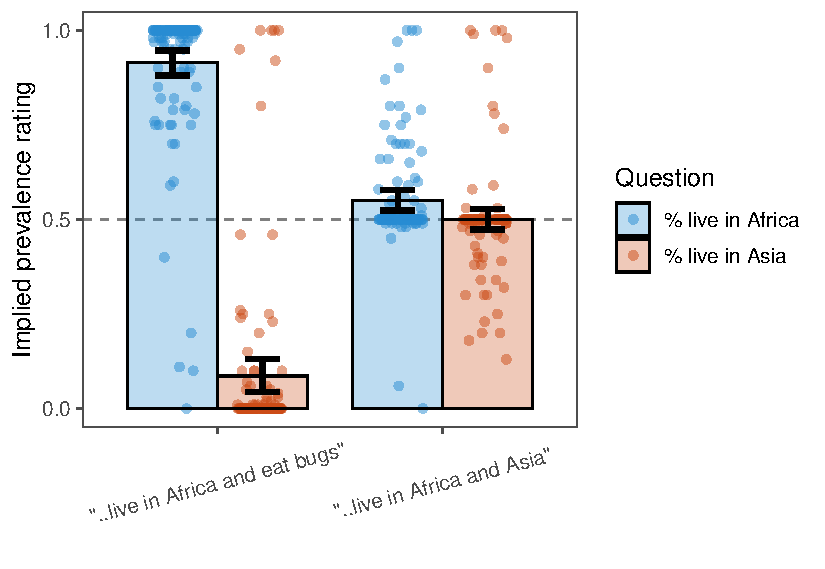
\includegraphics[width=0.5\textwidth]{expt1_summary}
    \vspace{-1cm}
  \caption{Experiment 1 results. Participants' ratings of the percentage of a category with a property (color) upon hearing a conjunctive generic either with non-mutually exclusive properties (left) or mutually exclusive properties (right).}
\end{figure}

\subsection{Experiment 2: Interrupting questions}

In Expt.~1, we observed that the nature of the second conjunct in a conjunctive generic sentence can influence inferences about the prevalence of the first conjunct.
Here, we test for a potential confound in the design of Expt.~1: Whenever participants provided prevalence estimates for two properties that they had read about in a conjunctive generic, the inference was that they were mutually exclusive. 
Here we provide a control wherein participants can provide ratings about two properties previously mentioned in a conjunctive generic but which are not  mutually exclusive. 
In addition, we aim to replicate the pattern of Expt.~1 using a gating technique wherein participants are queried part-way through a sentence. 

\subsubsection{Participants}

We recruited \red{N} participants through Amazon's Mechanical Turk.
This number was arrived at with the aim of collecting \red{N} participants' data who passed the attention checks.  
Participants were restricted to those with verified U.S. IP addresses and had at least a 95\% work approval rating. 

\subsubsection{Materials and procedure}

The materials were the same as used in Expt.~1. 

\subsubsection{Results}

\begin{figure}[h]
  \centering
    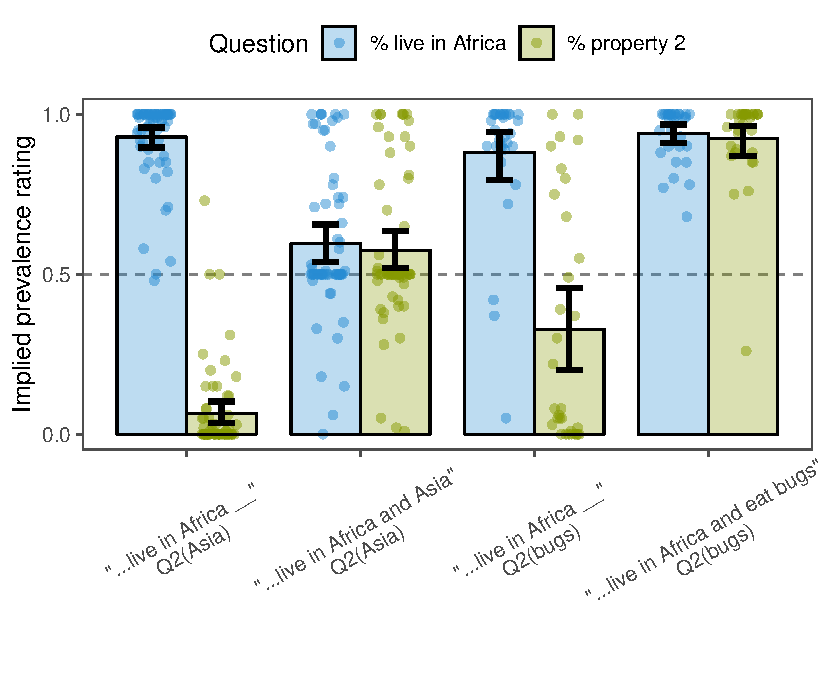
\includegraphics[width=0.5\textwidth]{expt2_summary}
%    \vspace{-1cm}
  \caption{Experiment 2 results. Property 2 is either the mutually exclusive property (left two bars) or non-mutually exclusive property (right two bars). ``\_\_'' indicates the question appears mid-sentence}
  \end{figure}

\subsection{Experiment 3: Interrupting questions}

In Expt.~2, we replicated the mutually-exclusive inference effects of Expt.~1 using a gating paradigm wherein participants are queried for their beliefs partway through a sentence. 
Here, we exploit this paradigm to test the incremental processing predictions of the model, wherein syntactic expectations can modulate the interpretations of generic sentences. 

\subsubsection{Participants}

We recruited \red{N} participants through Amazon's Mechanical Turk.
This number was arrived at with the aim of collecting \red{N} participants' data who passed the attention checks.  
Participants were restricted to those with verified U.S. IP addresses and had at least a 95\% work approval rating. 

\subsubsection{Materials}

\subsubsection{Procedure}
\begin{figure}[h]
  \centering
    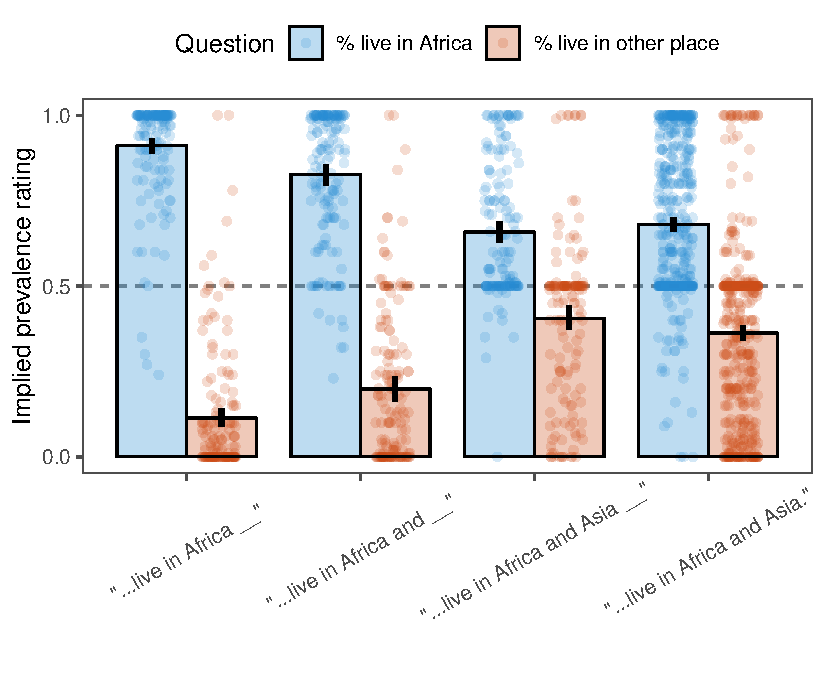
\includegraphics[width=0.5\textwidth]{expt3_summary}
%    \vspace{-1cm}
  \caption{Experiment 3 results.}
  \end{figure}

\section{Discussion}

\section{Acknowledgments}

We thank Karen Gu for her assistance in stimuli creation and experiment implementation.


\bibliographystyle{apacite}

\setlength{\bibleftmargin}{.125in}
\setlength{\bibindent}{-\bibleftmargin}

\bibliography{elephants}


\end{document}
